\input{\string~/Documents/School/"UC Irvine"/ta_template2.0.tex}
\rh{2B}{6.1}
\chead{\today}
\graphicspath{ {\string~/Desktop} }
\usetikzlibrary{arrows}
%============ANSWER KEY TOGGLE===========
\newcommand{\ans}[1]{ \noindent {\color{red} \textbf{Answer:} #1}}
%\renewcommand{\ans}[1]{\vspace{3in}}
%==========================================
\begin{document}
\begin{center}
\textbf{Area Between Curves}
\end{center}

\begin{prop}
The area between the curves $y = f(x)$ and $y =g(x)$ between $x = a$ and $x = b$ is given by:
\[
\int_a^b \lrabs{f(x) - g(x)}dx
\]
\end{prop}
\begin{aun}
Problems like these often involve integrating an absolute value symbol, which can be tricky! Remember to sort the interval $[a,b]$ into the regions where $f(x) \geq g(x)$ and $f(x) \leq g(x)$.
\end{aun}
\begin{exx}
Compute the area between the curves:
\[
f(x) = 4x - x^2 \mte{and} g(x) = x^2
\]
\end{exx}

\begin{center}
	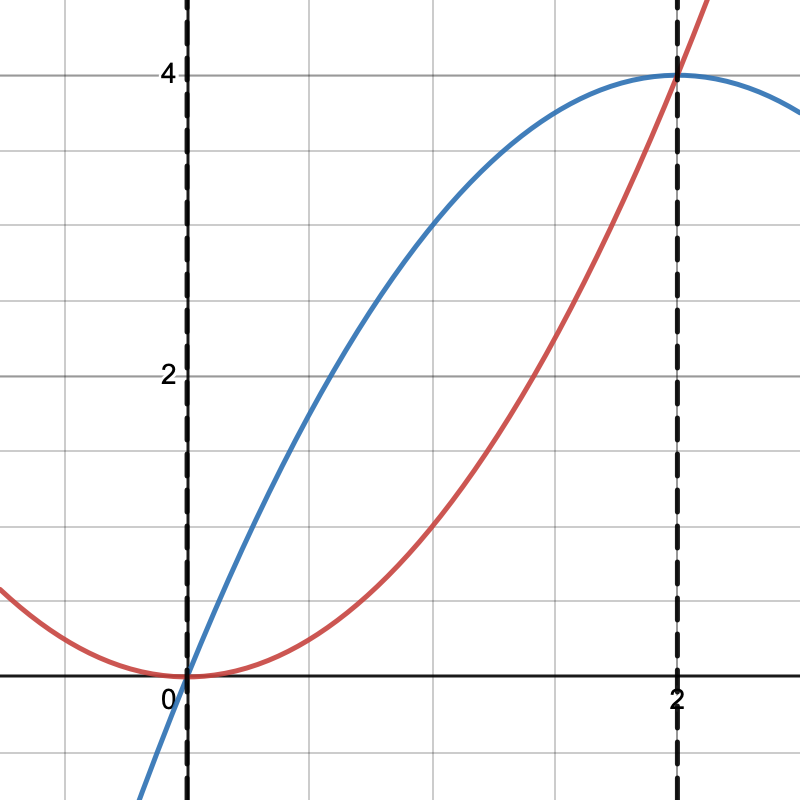
\includegraphics[width=0.25 \textwidth]{graph1.png}
\end{center}

\ans{From the image, we know that the correct integral to set up is:
\[
\int_0^2 f(x) - g(x) dx = 2 \int_0^2 2x - x^2 dx = 2 \lrb{x^2 - \frac{x^3}{3}}_0^2 = 2 \lrp{4 - \frac83} = \frac83
\]
}

\problembox{Compute the area between the curves:
\[
f(x) = \frac{8}{x}, \mte{  } g(x) = 2x, \mte{ and } x = 4.
\]
Graph the region in the grid below. 
}
\begin{center}
\tikzset{every picture/.style={line width=0.75pt}} %set default line width to 0.75pt        


\begin{tikzpicture}[x=0.75pt,y=0.75pt,yscale=-1,xscale=1]
%uncomment if require: \path (0,300); %set diagram left start at 0, and has height of 300

%Shape: Grid [id:dp6152831183024202] 
\draw  [draw opacity=0] (193,21) -- (414,21) -- (414,222) -- (193,222) -- cycle ; \draw   (193,21) -- (193,222)(213,21) -- (213,222)(233,21) -- (233,222)(253,21) -- (253,222)(273,21) -- (273,222)(293,21) -- (293,222)(313,21) -- (313,222)(333,21) -- (333,222)(353,21) -- (353,222)(373,21) -- (373,222)(393,21) -- (393,222)(413,21) -- (413,222) ; \draw   (193,21) -- (414,21)(193,41) -- (414,41)(193,61) -- (414,61)(193,81) -- (414,81)(193,101) -- (414,101)(193,121) -- (414,121)(193,141) -- (414,141)(193,161) -- (414,161)(193,181) -- (414,181)(193,201) -- (414,201)(193,221) -- (414,221) ; \draw    ;
\end{tikzpicture}
\end{center}

\ans{First we graph:
\[
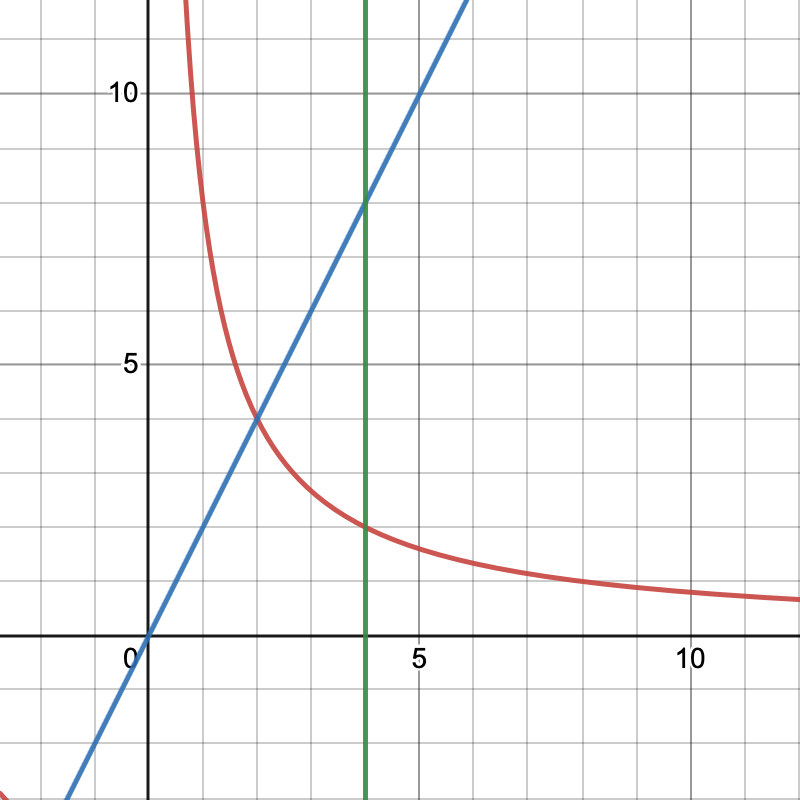
\includegraphics[width=0.5\textwidth]{graph2.png}
\]
and integrate:
\[
\int_2^4 2x - \frac8x dx = \lrb{x^2 - 8\ln(x)}_2^4
\]
}

\problembox{Sketch the region enclosed by the following curves, and then \textbf{set up an integral to} compute the area of these regions:
\[
y=x \sqrt{x^2+1}, y=e^{-\frac{1}{2} x}, x=-3  \mte{and the} y\text{-axis.}
\]
}
\begin{center}
\tikzset{every picture/.style={line width=0.75pt}} %set default line width to 0.75pt        


\begin{tikzpicture}[x=0.75pt,y=0.75pt,yscale=-1,xscale=1]
%uncomment if require: \path (0,300); %set diagram left start at 0, and has height of 300

%Shape: Grid [id:dp6152831183024202] 
\draw  [draw opacity=0] (193,21) -- (414,21) -- (414,222) -- (193,222) -- cycle ; \draw   (193,21) -- (193,222)(213,21) -- (213,222)(233,21) -- (233,222)(253,21) -- (253,222)(273,21) -- (273,222)(293,21) -- (293,222)(313,21) -- (313,222)(333,21) -- (333,222)(353,21) -- (353,222)(373,21) -- (373,222)(393,21) -- (393,222)(413,21) -- (413,222) ; \draw   (193,21) -- (414,21)(193,41) -- (414,41)(193,61) -- (414,61)(193,81) -- (414,81)(193,101) -- (414,101)(193,121) -- (414,121)(193,141) -- (414,141)(193,161) -- (414,161)(193,181) -- (414,181)(193,201) -- (414,201)(193,221) -- (414,221) ; \draw    ;
\end{tikzpicture}
\end{center}
\ans{Show students here that it's not necessary to know the exact shape of a graph so long as they can find intersection points and know the region of integration.
\[
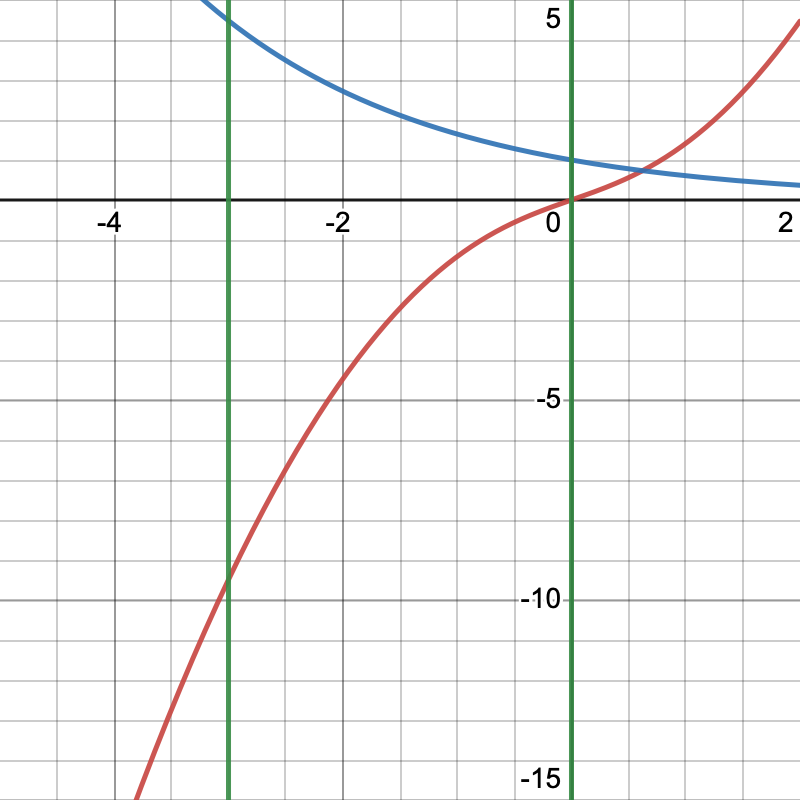
\includegraphics[width=0.5\textwidth]{graph3.png}
\]
The correct integral would be:
\[
\int_{-3}^0 e^{- \frac12 x} - x \sqrt{x^2+1} dx
\]
}

\end{document}